\documentclass[conference]{IEEEtran}
\IEEEoverridecommandlockouts

\usepackage{cite}
\usepackage{amsmath,amssymb,amsfonts}
\usepackage{graphicx}
\usepackage{textcomp}
\usepackage{xcolor}
\usepackage{booktabs}
\usepackage{multirow}
\usepackage{url}

\def\BibTeX{{\rm B\kern-.05em{\sc i\kern-.025em b}\kern-.08em
    T\kern-.1667em\lower.7ex\hbox{E}\kern-.125emX}}
\makeatletter
\newcommand{\linebreakand}{%
  \end{@IEEEauthorhalign}
  \hfill\mbox{}\par
  \mbox{}\hfill\begin{@IEEEauthorhalign}
}
\makeatother
\begin{document}

\title{Apparent Inefficiency, Hidden Optimality: Why the Brain's Multimodal Attention Does Not Track Feature Strength}

\author{
\IEEEauthorblockN{Xiaoyue Ding}
\IEEEauthorblockA{\textit{Faculty of Psychology} \\
\textit{Beijing Normal University}\\
Beijing, China \\
dingxiaoyue0327@163.com}
\and
\IEEEauthorblockN{Cuicui Jiang}
\IEEEauthorblockA{\textit{College of Computer Science} \\
\textit{Inner Mongolia University}\\
Hohhot, China \\
jiangcuicui@mail.imu.edu.cn}
\and
\IEEEauthorblockN{Rumei Yang}
\IEEEauthorblockA{\textit{School of Nursing} \\
\textit{Nanjing Medical University}\\
Nanjing, China \\
rumeiyang@njmu.edu.cn}
\linebreakand
\IEEEauthorblockN{Jiaoping Chen}
\IEEEauthorblockA{\textit{Merrick School of Business} \\
\textit{University of Baltimore}\\
Baltimore, MD, USA \\
jchen@ubalt.edu}
\and
\IEEEauthorblockN{Xiaoyan Li\textsuperscript{*}}
\IEEEauthorblockA{\textit{Dept. of Computational Mathematics,} \\
\textit{Science and Engineering} \\
\textit{Michigan State University}\\
East Lansing, MI, USA \\
lixiaoy5@msu.edu \\
\textsuperscript{*}\textit{Corresponding author}}
\and
\IEEEauthorblockN{Yujia Du}
\IEEEauthorblockA{\textit{Suzhou MetaCortex Intelligence} \\
\textit{Technology Co., Ltd.}\\
Suzhou, China \\
saroyi@163.com}
}

\maketitle

\begin{abstract}
How does the brain allocate attention across sensory modalities during multimodal integration? Classical Bayesian frameworks predict that efficient systems weight each modality in proportion to its encoding strength. We tested this prediction using fMRI data from four participants watching naturalistic movies (~65 hours). Through unimodal encoding models and a personalized multimodal neural network with learnable modality weights, we found a striking dissociation: visual features dominated encoding (mean $r = 0.204$, 91\% of brain regions), yet the learned attention weights remained balanced ($\sim$33\% per modality). We term this the Encoding-Attention Dissociation. The finding persisted when restricting analysis to high-encoding regions ($r > 0.2$, 407 regions), under end-to-end retraining, and with alternative feature extractors (CLIP, Wav2Vec2, GPT-2). The Default Mode Network emerged as the primary integration hub (Multimodal Integration Index = 0.744), with integration following a gradient from sensory to transmodal cortex. These results are consistent with the possibility that multimodal integration in the brain favors robustness over narrow efficiency, maintaining balanced attention regardless of encoding strength.
\end{abstract}

\begin{IEEEkeywords}
multimodal integration, encoding models, attention allocation, fMRI, Default Mode Network, robust optimization
\end{IEEEkeywords}

\section{Introduction}

Multimodal integration is central to human cognition, enabling us to effortlessly understand naturalistic environments by binding visual, auditory, and linguistic information. How the brain achieves this integration, and how it allocates attentional resources across modalities, remains a fundamental question in computational neuroscience \cite{stein1993merging, beauchamp2004unraveling}.

A foundational view holds that the brain integrates multisensory signals in a statistically optimal manner, weighting each source according to its reliability \cite{ernst2002humans, knill2004bayesian}. This framework predicts that more reliable signals receive proportionally greater weight, as confirmed in visual-haptic \cite{ernst2002humans} and visual-vestibular \cite{fetsch2013bridging} integration. However, balanced cross-modal attention can enhance performance compared to focusing on a single channel \cite{mishra2012attention}, suggesting a strategy more nuanced than proportional weighting.

Encoding models link stimulus features to brain activity \cite{naselaris2011encoding}: deep network hierarchies correspond to visual processing hierarchies \cite{gucclu2015deep}, language representations are distributed across cortex in organized gradients \cite{huth2016natural}, and large language model representations predict brain activity during language processing \cite{caucheteux2022brains}.

The human cerebral cortex is organized hierarchically from primary sensory regions to higher-order association areas \cite{margulies2016situating}, formalized in the Schaefer parcellation with seven functional networks spanning unimodal to transmodal processing \cite{schaefer2018local}. The Default Mode Network (DMN) occupies a unique position in this hierarchy, implicated in semantic integration, narrative comprehension, and mental simulation \cite{mar2011neural, simony2016dynamic}. This hierarchical organization motivates the question: does the transition from unimodal to multimodal processing follow a systematic gradient, and where does the brain implement multimodal attention allocation?

We propose and test three hypotheses about multisensory processing. First, modality-specific encoding in early sensory regions gives way to shared, amodal representations in higher-order cortices. Second, integration follows a hierarchical structure with the DMN serving as a primary integration hub. Third, and most critically, attention allocation during multisensory integration is decoupled from encoding strength, a principle we term the \textit{Encoding-Attention Dissociation}. The first two hypotheses build on established findings about cortical hierarchy \cite{margulies2016situating} and validate our framework; the novel contribution lies in the third hypothesis and its control analyses. Understanding the computational principles of multimodal integration has biomedical relevance: disrupted multisensory processing is implicated in autism spectrum disorder \cite{stevenson2014multisensory}, schizophrenia, and age-related cognitive decline, and quantitative characterization of normal integration strategies is a prerequisite for identifying pathological deviations.

\section{Methods}

\subsection{Data and Participants}

We used a naturalistic movie-watching paradigm because it provides concurrent visual, auditory, and linguistic stimulation under ecologically valid conditions, making it well suited for studying multimodal integration \cite{hasson2010reliability}. Functional MRI data were obtained from the Algonauts 2025 Challenge \cite{gifford2024algonauts}, derived from the Courtois NeuroMod project \cite{boyle2023courtois}. Four healthy adult participants viewed approximately 65 hours of movie content including the television series \textit{Friends} (seasons 1--6, 55 hours) for model training and validation (80\%/20\% split) and the Movie10 dataset (10 hours) as an independent test set. The fMRI data were acquired with a repetition time (TR) of 1.49\,s and parcellated into 1,000 cortical regions using the Schaefer atlas \cite{schaefer2018local}, which organizes the cortex into seven functional networks: Visual, Somatomotor, Dorsal Attention, Ventral Attention, Limbic, Frontoparietal, and Default Mode.

\subsection{Feature Extraction}

To extract stimulus representations, we employed one primary and one alternative model per modality to ensure findings generalize beyond any single feature extractor (see Section~\ref{sec:multimodel}). The primary models were: visual features from SlowFast 3D ResNet pretrained on Kinetics-400 \cite{feichtenhofer2019slowfast} (8,192 dimensions); auditory features from 20-dimensional mel-frequency cepstral coefficients (MFCCs); and language features from contextualized BERT embeddings \cite{devlin2019bert} (768 dimensions, 10 tokens per TR). Feature dimensionality was reduced via principal component analysis (PCA) to 250 components for visual and language features and 20 components for audio, with PCA models fit on training data only.

To account for hemodynamic delays, stimulus features were temporally aligned to fMRI acquisitions using a sliding window approach:
\begin{equation}\label{eq:xt}
\mathbf{x}_t^{(m)} = \sum_{\tau=0}^{T_w-1} h(\tau) \cdot \mathbf{f}_{t-\delta-\tau}^{(m)}
\end{equation}
where $\mathbf{f}^{(m)}$ denotes the feature vector for modality $m$, $h(\tau)$ is the canonical HRF kernel, $\delta = 3$ TRs is the hemodynamic delay, and $T_w = 5$ TRs is the temporal integration window.

\subsection{Unimodal Encoding Models}

For each participant, modality, and brain region, we trained Ridge regression encoding models with 5-fold cross-validation for regularization parameter selection from a logarithmic grid spanning $10^{-3}$ to $10^{6}$:
\begin{equation}\label{eq:L}
\mathcal{L}(\boldsymbol{\beta}) =
\lVert \mathbf{y} - \mathbf{X}\boldsymbol{\beta} \rVert_2^2
+ \lambda \lVert \boldsymbol{\beta} \rVert_2^2
\end{equation}
where $\mathbf{y} \in \mathbb{R}^N$ is the fMRI time series, $\mathbf{X} \in \mathbb{R}^{N \times D}$ is the feature matrix, and $\lambda$ is the regularization parameter. Encoding performance was quantified using Pearson correlation $r = \mathrm{corr}(\hat{\mathbf{y}}, \mathbf{y})$. Ridge regression is the standard, interpretable choice in the encoding literature \cite{naselaris2011encoding}.

\subsection{Personalized Multimodal Neural Network}

To disentangle modality-specific encoding strength from cross-modal attention allocation, we developed a hierarchical multimodal neural architecture. Each modality $m \in \{V, A, L\}$ is processed through a dedicated encoder (two-layer MLP with BatchNorm and dropout), producing a shared 512-dimensional representation. The three modality representations are integrated via multi-head cross-modal attention \cite{vaswani2017attention} (8 heads). Critically, multimodal fusion is governed by explicit learnable modality weights $\boldsymbol{\alpha} = (\alpha_V, \alpha_A, \alpha_L)$, normalized via softmax, which determine the relative contribution of each modality and are learned jointly with all other parameters. Subject-specific adapter networks account for inter-individual variability. The model was trained end-to-end using the Adam optimizer (learning rate $10^{-4}$, batch size 32) with early stopping based on validation loss (patience = 10 epochs). A neural network rather than Ridge regression was used for fusion because nonlinear cross-modal interactions require learnable attention mechanisms.

\subsection{Quantitative Indices}

\subsubsection{Modality Specificity Index (MSI)}
To quantify the degree to which a brain region preferentially encodes one modality, inspired by selectivity indices in neurophysiology \cite{desimone1984stimulus}:
\begin{equation}\label{eq:msi}
MSI_i = \frac{r_i^{\max} - \bar{r}_i^{\text{other}}}{r_i^{\max} + \bar{r}_i^{\text{other}}}
\end{equation}
where $r_i^{\max}$ is the highest encoding correlation and $\bar{r}_i^{\text{other}}$ is the mean of the remaining two. Values range from 0 (balanced) to 1 (perfectly specific).

\subsubsection{Multimodal Integration Index (MII)}
To quantify the balance of multimodal encoding at the network level:
\begin{equation}\label{eq:mii}
MII_n = 1 - \frac{\sigma_n(r_V, r_A, r_L)}{\mu_n(r_V, r_A, r_L)}
\end{equation}
where $\sigma_n$ and $\mu_n$ are the standard deviation and mean of encoding correlations within network $n$. Higher MII indicates more balanced integration.

\subsubsection{Efficiency Gap}
To directly test the Encoding-Attention Dissociation:
\begin{equation}\label{eq:delta}
\Delta_m = \alpha_m^{\text{eff}} - \alpha_m^{\text{obs}}, \quad \alpha_m^{\text{eff}} = \frac{r_m}{\sum_{m'} r_{m'}}
\end{equation}
where $\alpha_m^{\text{obs}}$ is the learned attention weight and $\alpha_m^{\text{eff}}$ is the weight that would result from proportional allocation. A positive gap for the dominant modality indicates systematic under-weighting of strong signals.

\subsection{Statistical Analysis}

Network-level modality differences were assessed using one-way ANOVA with Bonferroni correction ($\alpha = 0.05$, 21 comparisons). Cross-subject consistency was quantified using the intraclass correlation coefficient ICC(1,1) \cite{shrout1979intraclass}.

\section{Results}

\subsection{Visual Encoding Dominates Sensory Regions}

Before testing whether attention tracks encoding strength (Hypothesis~3), we first need to establish that a clear encoding asymmetry exists across modalities. Ridge regression encoding models revealed that visual features produced the highest encoding accuracy across all participants (Table~\ref{tab:encoding}), with visual features achieving approximately twice the encoding strength of auditory and language features. Visual encoding dominated 91\% of the 1,000 cortical regions (Fig.~\ref{fig:Fig1}a--d). However, the extent of visual dominance varied across networks: the Visual network exhibited the strongest visual encoding, while the DMN showed more balanced encoding profiles (Fig.~\ref{fig:Fig1}f). One-way ANOVA confirmed significant modality differences within each network, with visual dominance decreasing along the sensory-to-transmodal cortical gradient. These results agree with established findings on modality-specific processing \cite{gucclu2015deep}.

\begin{table}[t]
\caption{Unimodal Encoding Performance (Pearson $r$). Mean encoding correlation across 1{,}000 Schaefer parcels per participant and modality. Bold: highest-encoding modality per row.}
\label{tab:encoding}
\centering
\setlength{\tabcolsep}{8pt}
\begin{tabular}{lccc}
\toprule
Subject & Visual & Audio & Language \\
\midrule
Sub-01 & \textbf{0.214} & 0.112 & 0.129 \\
Sub-02 & \textbf{0.195} & 0.102 & 0.130 \\
Sub-03 & \textbf{0.220} & 0.118 & 0.119 \\
Sub-05 & \textbf{0.186} & 0.095 & 0.110 \\
\midrule
Mean & \textbf{0.204} & 0.107 & 0.122 \\
\bottomrule
\end{tabular}
\end{table}

\begin{figure*}[t]
    \centering
    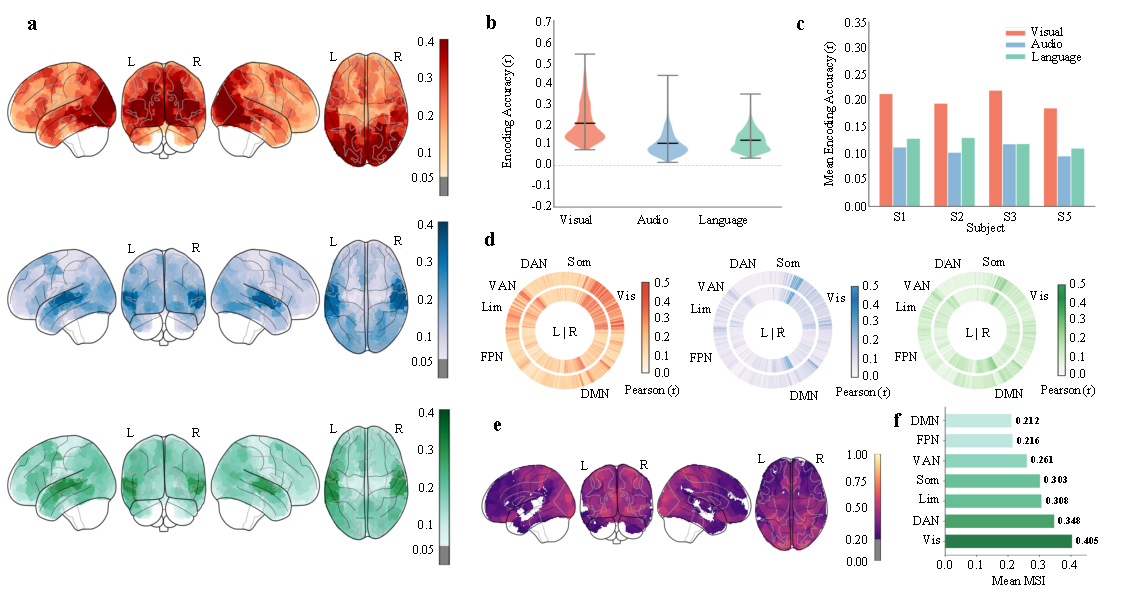
\includegraphics[width=0.85\textwidth]{figure1.pdf}
    \caption{\textbf{Unimodal encoding across modalities and brain networks.}
    \textbf{a,} Cortical maps of unimodal encoding strength (Pearson $r$, averaged across participants); rows: visual, audio, language.
    \textbf{b,} Distribution of encoding $r$ across 1{,}000 parcels pooled across participants (means: V$=0.204$, A$=0.107$, L$=0.122$).
    \textbf{c,} Per-participant mean $r$ across all 1{,}000 parcels for each modality.
    \textbf{d,} Mean encoding $r$ within each Schaefer network, per modality.
    \textbf{e,} Cortical maps of the Modality Specificity Index (MSI; Eq.~\ref{eq:msi}; 0 = balanced, 1 = exclusive).
    \textbf{f,} Network-level mean MSI ranked from most modality-specific to most balanced.}
    \label{fig:Fig1}
\end{figure*}

\subsection{Hierarchical Organization with the DMN as Integration Hub}

Having established the encoding asymmetry, we next ask \textit{where} multimodal integration occurs. If integration follows a hierarchical architecture with dedicated hub regions, this could provide the structural basis for an attention allocation mechanism that operates independently of encoding strength. The Multimodal Integration Index (MII) revealed a systematic gradient: the Visual network exhibited the lowest MII while the DMN exhibited the highest ($MII = 0.744$), reflecting balanced multimodal processing (Fig.~\ref{fig:Fig2}a,b). This hierarchy was consistent across participants (ICC = 0.89) and aligned with the known unimodal-to-transmodal cortical gradient \cite{margulies2016situating}. Hierarchical clustering of brain regions by their multimodal encoding profiles showed an above-chance but partial correspondence with the canonical networks (adjusted Rand index 0.11 for seven clusters; label-shuffle 95th percentile 0.007; Fig.~\ref{fig:Fig2}c). The group-average functional connectivity matrix (1,407 runs) confirmed the network partition used in these analyses: within-network connectivity (mean $r = 0.12$) exceeded between-network connectivity (mean $r = 0.01$; network-level $t(26) = 6.4$, $p < 0.001$; Fig.~\ref{fig:Fig2}d).


\subsection{The Encoding-Attention Dissociation}

We now test the central question: does the brain's attention allocation track the encoding asymmetry? If the brain followed an ``efficient'' feature-tracking strategy, attention weights should be proportional to encoding accuracy. Given visual features' $\sim$2$\times$ encoding advantage, an efficient allocation would assign approximately 47\% to visual, 28\% to language, and 25\% to audio. However, the learned attention weights from our multimodal network revealed a strikingly different pattern.

Table~\ref{tab:attn_per_subject} presents the per-subject attention weights. All four participants exhibited nearly identical balanced weights ($\sim$33\% per modality), with cross-subject standard deviations below 0.002 for each modality. The models converged via early stopping between epochs 11--13, and achieved meaningful encoding performance on the validation set (mean $r$ = 0.117--0.138, with 480--618 regions exceeding $r > 0.1$), confirming that the learned weights reflect genuine stimulus--brain relationships rather than noise.

Table~\ref{tab:dissociation} summarizes the Encoding-Attention Dissociation at the group level. The Efficiency Gap for visual was $+14.8\%$, meaning the brain under-weights its strongest modality by nearly one-third relative to what proportional allocation would predict. Conversely, audio and language are over-weighted by 9.8\% and 5.0\%, respectively.

\begin{table}[t]
\caption{Per-Subject Attention Weights from the Multimodal Network. Attention weights $\alpha$: softmax-normalized modality weights (sum to 1 per row). Validation on held-out Friends S6 + Movie10. ``Mean $r$'': cross-parcel mean encoding correlation; ``$r > 0.1$'': count of parcels (out of 1{,}000) exceeding that correlation.}
\label{tab:attn_per_subject}
\centering
\begin{tabular*}{\columnwidth}{@{\extracolsep{\fill}}lcccccc@{}}
\toprule
 & \multicolumn{3}{c}{Attention Weight $\alpha$} & \multicolumn{2}{c}{Val.\ Performance} \\
\cmidrule(lr){2-4} \cmidrule(lr){5-6}
Subject & Visual & Audio & Lang. & Mean $r$ & $r\!>\!0.1$ \\
\midrule
Sub-01 & 0.324 & 0.343 & 0.333 & 0.138 & 618 \\
Sub-02 & 0.321 & 0.347 & 0.331 & 0.128 & 554 \\
Sub-03 & 0.325 & 0.346 & 0.329 & 0.138 & 538 \\
Sub-05 & 0.323 & 0.347 & 0.331 & 0.117 & 480 \\
\midrule
Mean & 0.323 & 0.346 & 0.331 & 0.130 & 548 \\
SD & 0.001 & 0.002 & 0.001 & --- & --- \\
\bottomrule
\end{tabular*}
\end{table}

\begin{table}[t]
\caption{Encoding-Attention Dissociation (Group-Level Summary). Encoding $r$: group mean across participants and parcels. Efficient $\alpha = r_m / \sum r_{m'}$ (Bayesian prediction, Eq.~\ref{eq:delta}). Observed $\alpha$: weight learned by the multimodal network. Efficiency Gap $= \alpha^{\text{eff}} - \alpha^{\text{obs}}$ (positive = under-weighting).}
\label{tab:dissociation}
\centering
\setlength{\tabcolsep}{8pt}
\begin{tabular}{lccc}
\toprule
 & Visual & Audio & Language \\
\midrule
Encoding $r$ & \textbf{0.204} & 0.107 & 0.122 \\
Efficient $\alpha$ & 47.1\% & 24.7\% & 28.2\% \\
Observed $\alpha$ & 32.3\% & 34.6\% & 33.1\% \\
Efficiency Gap & $+$14.8\% & $-$9.8\% & $-$5.0\% \\
\bottomrule
\end{tabular}
\end{table}

\begin{figure*}[t]
    \centering
    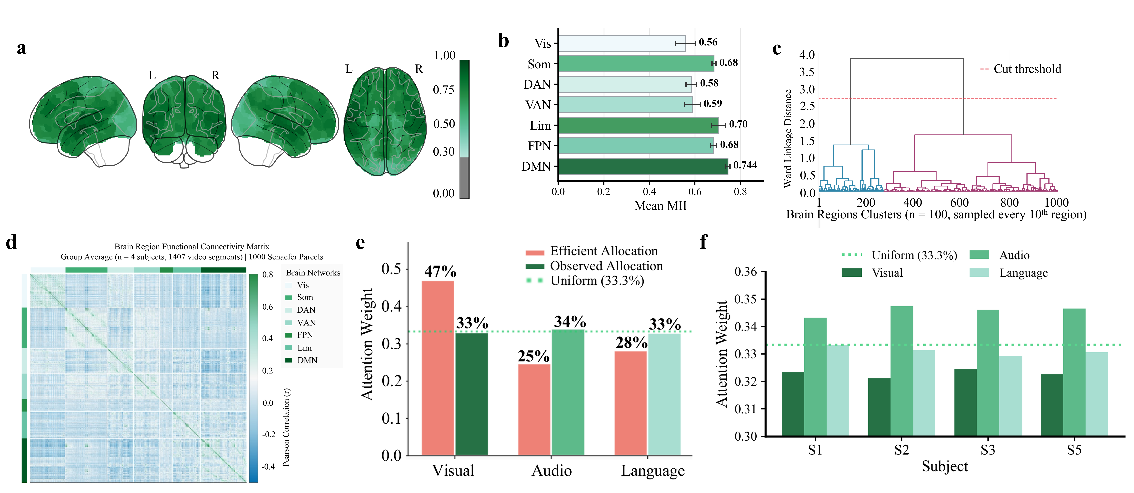
\includegraphics[width=0.85\textwidth]{figure2.pdf}
    \caption{\textbf{Hierarchical integration and Encoding-Attention Dissociation.}
    \textbf{a,} Cortical maps of the Multimodal Integration Index (MII; Eq.~\ref{eq:mii}; higher = more balanced).
    \textbf{b,} Network-level mean MII; DMN highest ($MII = 0.744$), Visual lowest. Error bars: SD across participants; $\text{ICC}(1,1) = 0.89$.
    \textbf{c,} Ward hierarchical clustering of parcels by encoding profile ($r_V, r_A, r_L$).
    \textbf{d,} Group-average functional connectivity between parcels (BOLD correlation, Fisher-$z$ averaged over 1{,}407 runs).
    \textbf{e,} Efficient ($\alpha^{\text{eff}}_m = r_m / \sum r_{m'}$; Eq.~\ref{eq:delta}, left) vs.\ observed (right) attention weights. Efficient predicts $47\%$ visual; observed is balanced near $33\%$.
    \textbf{f,} Per-participant observed weights; cross-subject SD $< 0.002$. Dotted line: uniform allocation ($\alpha = 1/3$).}
    \label{fig:Fig2}
\end{figure*}

\subsection{Control Analyses}\label{sec:controls}

Could the dissociation arise from methodological artifacts? Three alternative explanations must be addressed: (1)~the multimodal model fits poorly, so weights default to uniform; (2)~the training procedure constrains weights to remain balanced; (3)~the encoding asymmetry is specific to the chosen feature models, not the modalities themselves. We conducted a targeted control analysis for each.

\subsubsection{High-Encoding Subset Analysis}
If balanced weights merely reflect poor model fit, restricting analysis to well-predicted regions should alter the pattern. We retrained the multimodal network three times, each time including only brain regions where the best unimodal encoding exceeded a threshold: $r > 0.1$, $r > 0.15$, and $r > 0.2$.

Table~\ref{tab:subset_detail} presents per-subject results at each threshold. Even at the strictest threshold ($r > 0.2$), which retains only 333--465 of 1,000 regions per subject, the attention weights remained balanced. Strikingly, the weights became \textit{more} balanced at higher thresholds (Fig.~\ref{fig:Fig3}a): the coefficient of variation (CV) of the three modality weights decreased from 0.036 at $r > 0.1$ to 0.011 at $r > 0.2$. This means the dissociation is strongest precisely in the brain regions where encoding models perform best, directly contradicting the poor-fit explanation.

\begin{table*}[t]
\caption{Per-Subject Control Results. Subset conditions: the multimodal network was retrained using only parcels with $\max(r_V, r_A, r_L) >$ threshold; $n$: surviving parcel count (out of 1{,}000). E2E: full model retrained with learning rate halved to $5 \times 10^{-5}$; Val.\ $r$: validation mean $r$ across 1{,}000 parcels. V/A/L: softmax-normalized modality weights.}
\label{tab:subset_detail}
\centering
\footnotesize
\setlength{\tabcolsep}{3.2pt}
\begin{tabular*}{\textwidth}{@{\extracolsep{\fill}}l cccc cccc cccc cccc@{}}
\toprule
 & \multicolumn{4}{c}{Subset $r\!>\!0.1$} & \multicolumn{4}{c}{Subset $r\!>\!0.15$} & \multicolumn{4}{c}{Subset $r\!>\!0.2$} & \multicolumn{4}{c}{E2E (lr $=5\!\times\!10^{-5}$)} \\
\cmidrule(lr){2-5}\cmidrule(lr){6-9}\cmidrule(lr){10-13}\cmidrule(lr){14-17}
Subject & $n$ & V & A & L & $n$ & V & A & L & $n$ & V & A & L & Val.\ $r$ & V & A & L \\
\midrule
Sub-01 & 944 & 0.327 & 0.344 & 0.329 & 715 & 0.328 & 0.342 & 0.331 & 448 & 0.333 & 0.334 & 0.334 & 0.137 & 0.329 & 0.342 & 0.329 \\
Sub-02 & 929 & 0.325 & 0.346 & 0.329 & 627 & 0.326 & 0.344 & 0.330 & 383 & 0.330 & 0.336 & 0.334 & 0.128 & 0.326 & 0.344 & 0.330 \\
Sub-03 & 982 & 0.325 & 0.346 & 0.330 & 695 & 0.325 & 0.345 & 0.331 & 465 & 0.327 & 0.337 & 0.336 & 0.128 & 0.329 & 0.342 & 0.329 \\
Sub-05 & 928 & 0.324 & 0.347 & 0.330 & 549 & 0.331 & 0.337 & 0.332 & 333 & 0.331 & 0.336 & 0.333 & 0.100 & 0.327 & 0.345 & 0.329 \\
\bottomrule
\end{tabular*}
\end{table*}

\subsubsection{End-to-End Training Control}
If balanced weights were an artifact of the training procedure (for example, if the learning rate were too high for the modality weights to differentiate), then changing the training configuration should alter the result. We retrained the full model for all four subjects using a lower learning rate ($5 \times 10^{-5}$, halved from the standard $10^{-4}$), allowing finer-grained gradient updates to the modality weight parameters. As shown in Table~\ref{tab:subset_detail} (E2E columns), the resulting weights remained balanced across all subjects (mean: V = 0.328, A = 0.343, L = 0.329), confirming that the finding is not sensitive to training hyperparameters.


\subsubsection{Multi-Model Feature Robustness}\label{sec:multimodel}
A critical concern is whether visual dominance reflects the specific feature extractors (e.g., unusually brain-predictive SlowFast features or unusually poor MFCCs) rather than the modalities themselves.

To address this, we extracted features using an entirely independent set of models: CLIP ViT-B/32 \cite{radford2021learning} for visual features (768D, pretrained on image-text pairs), Wav2Vec2-base \cite{baevski2020wav2vec} for audio (768D, self-supervised speech representations), and GPT-2 \cite{radford2019language} for language (768D, autoregressive language model). These models differ fundamentally from the primary models in architecture (transformer vs.\ CNN, self-supervised vs.\ supervised), training data, and output dimensionality.

Table~\ref{tab:multimodel_detail} and Fig.~\ref{fig:Fig3}b show per-subject encoding results for both feature sets. Despite these differences, the modality ordering was preserved in every subject: visual encoding consistently produced the highest correlation, followed by language, then audio. The visual-to-audio encoding ratio was 1.9$\times$ with primary models and 1.3$\times$ with alternative models: different in magnitude but consistent in direction. This confirms that visual encoding dominance is a property of the sensory modality during naturalistic movie viewing, not an artifact of any specific feature extraction model. Fig.~\ref{fig:Fig3}c visualizes the dissociation directly: under efficient allocation, each point (one per subject $\times$ modality) would fall on the diagonal; instead, all points cluster near the horizontal uniform line.

\begin{table}[t]
\caption{Multi-Model Encoding: Per-Subject Comparison. Each modality encoded by two architecturally distinct models: primary (SlowFast, MFCC, BERT) vs.\ alternative (CLIP, Wav2Vec2, GPT-2). Values: mean encoding $r$ across 1{,}000 parcels. Bold marks the dominant modality (visual), preserved across both model sets.}
\label{tab:multimodel_detail}
\centering
\begin{tabular*}{\columnwidth}{@{\extracolsep{\fill}}llcccc@{}}
\toprule
Modality & Model & S01 & S02 & S03 & S05 \\
\midrule
\multirow{2}{*}{Visual}
 & SlowFast & \textbf{0.214} & \textbf{0.195} & \textbf{0.220} & \textbf{0.186} \\
 & CLIP & \textbf{0.155} & \textbf{0.144} & \textbf{0.163} & \textbf{0.136} \\
\midrule
\multirow{2}{*}{Audio}
 & MFCC & 0.112 & 0.102 & 0.118 & 0.095 \\
 & Wav2Vec2 & 0.117 & 0.112 & 0.120 & 0.102 \\
\midrule
\multirow{2}{*}{Language}
 & BERT & 0.129 & 0.130 & 0.119 & 0.110 \\
 & GPT-2 & 0.128 & 0.131 & 0.133 & 0.110 \\
\bottomrule
\end{tabular*}
\end{table}


\begin{figure*}[t]
    \centering
    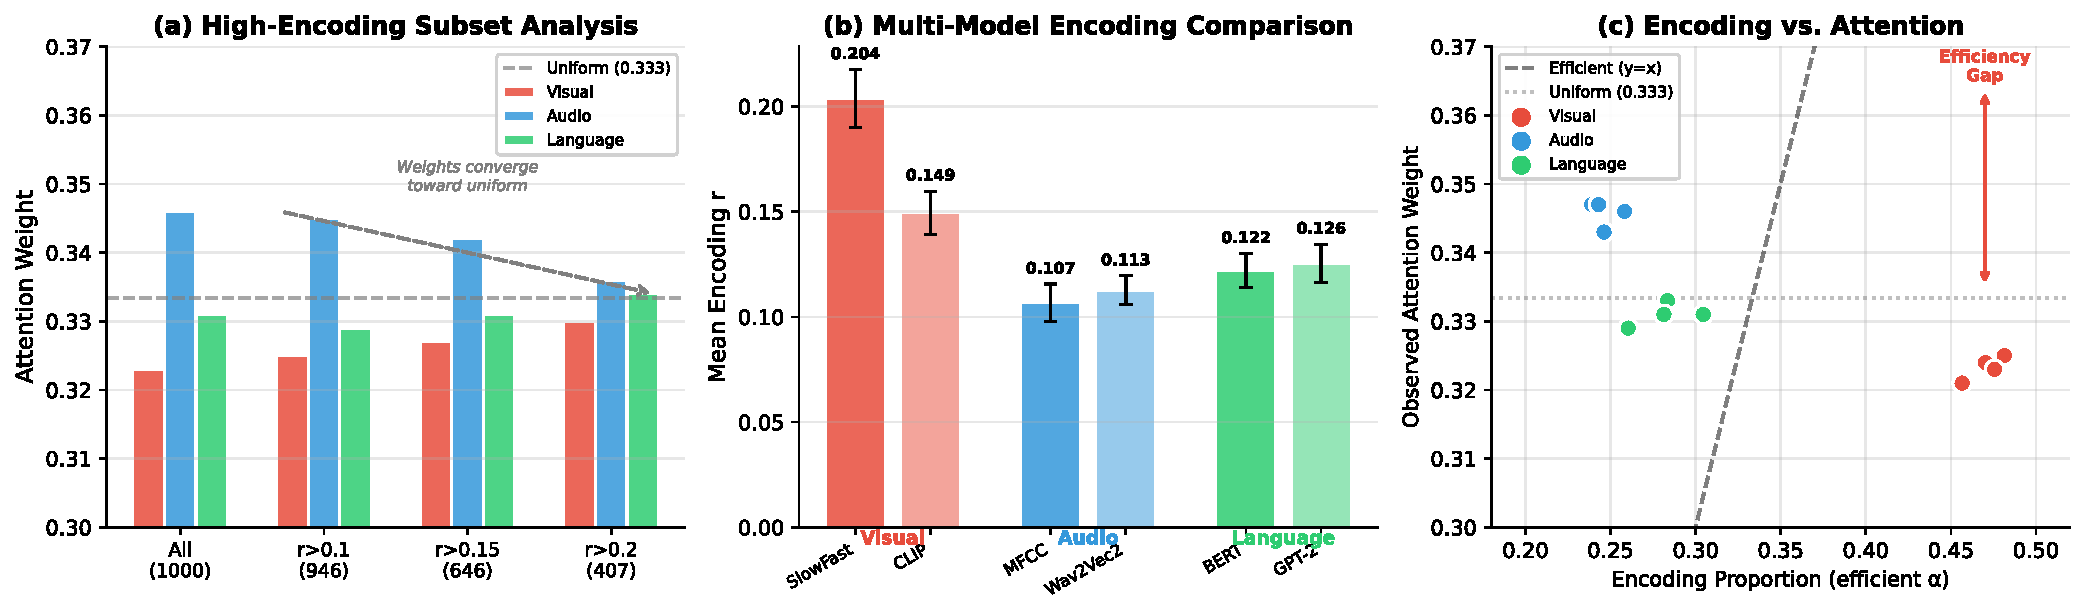
\includegraphics[width=\textwidth]{figure3_control_analyses.pdf}
    \caption{\textbf{Control analyses and multi-model validation.}
    \textbf{(a)} High-encoding subset analysis: as the threshold increases (fewer, better-predicted regions), weights converge toward uniform (dashed line).
    \textbf{(b)} Multi-model encoding comparison: mean encoding correlation ($\pm$ SD across subjects) for primary models (SlowFast, MFCC, BERT) and alternative models (CLIP, Wav2Vec2, GPT-2). The Visual $>$ Language $>$ Audio ordering is preserved across both model sets.
    \textbf{(c)} Encoding proportion vs.\ observed attention weight per subject $\times$ modality. Efficient allocation would place points on the diagonal (dashed); instead they cluster near the uniform line ($\alpha = 0.333$). The Efficiency Gap is largest for visual (red).}
    \label{fig:Fig3}
\end{figure*}

\subsection{Summary of Control Analyses}

Table~\ref{tab:controls_summary} synthesizes all conditions tested. Each row corresponds to a different potential confound: poor model fit (subset rows), training artifacts (E2E row), or model-specific effects (addressed by Table~\ref{tab:multimodel_detail}). In every case, attention weights remain within 1--2\% of the uniform distribution ($\frac{1}{3} \approx 0.333$). The maximum deviation across all 20 subject$\times$condition measurements was 2.3\%. Having ruled out three plausible alternative explanations, we interpret the Encoding-Attention Dissociation as reflecting a consistent property of multimodal integration in the participants studied, though replication with larger samples is needed.

\begin{table}[t]
\caption{Summary: Attention Weights Across All Conditions. Each row is one experimental condition; values are mean $\pm$ SD across the four participants. ``Standard'' is the main multimodal model (Table~\ref{tab:attn_per_subject}); ``Subset'' rows are the high-encoding subset control (Table~\ref{tab:subset_detail}); ``E2E'' is the lower-learning-rate control (Table~\ref{tab:subset_detail}). ``Uniform ref.'' is the theoretical $1/3$ reference for comparison, not a measurement.}
\label{tab:controls_summary}
\centering
\begin{tabular*}{\columnwidth}{@{\extracolsep{\fill}}lccc@{}}
\toprule
Condition & Visual & Audio & Language \\
\midrule
Standard & $0.323 \pm 0.001$ & $0.346 \pm 0.002$ & $0.331 \pm 0.001$ \\
Subset $r\!>\!0.1$ & $0.325 \pm 0.001$ & $0.345 \pm 0.001$ & $0.329 \pm 0.001$ \\
Subset $r\!>\!0.15$ & $0.327 \pm 0.002$ & $0.342 \pm 0.003$ & $0.331 \pm 0.001$ \\
Subset $r\!>\!0.2$ & $0.330 \pm 0.002$ & $0.336 \pm 0.001$ & $0.334 \pm 0.001$ \\
E2E (lr=$5\!\times\!10^{-5}$) & $0.328 \pm 0.001$ & $0.343 \pm 0.001$ & $0.329 \pm 0.001$ \\
\midrule
Uniform ref. & 0.333 & 0.333 & 0.333 \\
\bottomrule
\end{tabular*}
\end{table}

\section{Discussion}

\subsection{The Encoding-Attention Dissociation Challenges Bayesian Optimality}

Our results are consistent with all three hypotheses, and control analyses indicate that the Encoding-Attention Dissociation is not readily attributable to methodological artifacts. The central finding, that learned attention weights remain balanced at $\sim$33\% per modality despite a twofold visual encoding advantage, is at odds with the classical Bayesian framework predicting that attention tracks signal reliability \cite{ernst2002humans, knill2004bayesian}.

This dissociation is consistent with ecological rationality accounts \cite{gigerenzer2009homo}: when the informativeness of each modality varies across scenes, balanced attention may reduce the cost of unpredictable shifts. A visually uninformative but aurally rich scene (e.g., a dark screen during dialogue) would be poorly served by a visual-dominant strategy.

\subsection{Validity of Learned Weights as Attention Proxies}

Three observations support interpreting the learned modality weights as proxies for attention allocation. First, the model achieves meaningful prediction across 480--618 regions per subject ($r > 0.1$), indicating non-trivial stimulus--brain relationships \cite{kriegeskorte2008representational, yamins2016using}. Second, the weights are consistent across four independent participants (SD $< 0.002$ per modality). Third, the weights systematically diverge from encoding strength predictions in the same direction for all subjects, consistent with theoretical accounts of attention as a distinct selection mechanism separate from encoding \cite{lindsay2020attention}.

\subsection{Hierarchical Integration Architecture}

The MII gradient from the Visual network to the DMN aligns with the unimodal-to-transmodal cortical gradient \cite{margulies2016situating} and extends it to multimodal integration, not just representational content. The DMN's role as an integration hub is consistent with its function in narrative comprehension \cite{simony2016dynamic}, and balanced attention may be facilitated by its position atop the cortical hierarchy, where it operates on already-abstracted representations rather than raw sensory features.

\subsection{Biomedical Implications}

The Encoding-Attention Dissociation, if confirmed in larger populations, may have translational relevance. Atypical multisensory integration is a recognized feature of several clinical conditions: individuals with autism spectrum disorder show reduced temporal binding windows and altered modality weighting \cite{stevenson2014multisensory}, while patients with schizophrenia exhibit impaired audiovisual integration in speech perception \cite{ross2007impaired}. Quantifying the gap between encoding strength and attention allocation could serve as a computational biomarker for such deviations.

\subsection{Limitations}

Our sample size ($n = 4$) limits generalizability, though cross-subject consistency (ICC = 0.89) and replication across control conditions provide some confidence. The observed visual dominance may partly reflect the visual richness of professionally produced films rather than a universal property of multimodal processing. Audio-dominant or balanced audiovisual stimuli would test whether the dissociation generalizes. The correlational analysis precludes causal conclusions. The attention weights, while validated through multiple controls, remain an indirect proxy derived from a computational model; future work incorporating direct neural manipulations (e.g., TMS to the DMN) or behavioral attention measures would strengthen the mechanistic account. We also did not perform a formal permutation test of modality labels due to computational cost; a shuffled-label null distribution would provide additional statistical grounding for the dissociation. Finally, the alternative feature models, while architecturally distinct, all represent deep learning approaches; incorporating classical signal-processing features (e.g., Gabor filters for vision) could further strengthen the multi-model validation.

\section{Conclusion}

This study provides evidence for an Encoding-Attention Dissociation in multimodal processing: despite visual features dominating encoding in 91\% of cortical regions, learned attention weights remain balanced at approximately 33\% per modality. Control analyses spanning encoding thresholds, training configurations, and feature extraction models indicate that this pattern is not readily explained by methodological artifacts. The DMN serves as the primary integration hub within a hierarchical framework ascending from modality-specific sensory cortex. These findings are consistent with the possibility that the brain's apparent inefficiency in attention allocation reflects a strategy favoring robustness. Replication with larger samples and diverse stimulus paradigms will be important for establishing generality.

\section*{Acknowledgment}

This work used data from the Courtois NeuroMod project and the Algonauts 2025 Challenge (\url{https://algonautsproject.com/}). Code is available at \url{https://github.com/xiaoyanLi629/encoding-attention-dissociation}. The authors used Claude (Anthropic) to assist with analysis and figure-generation scripts, preparation of the camera-ready version, and language editing. The authors reviewed all AI-assisted content and take full responsibility for the paper.

\begin{thebibliography}{00}
\bibitem{stein1993merging} B.~E. Stein and M.~A. Meredith, \textit{The Merging of the Senses}. MIT Press, 1993.
\bibitem{beauchamp2004unraveling} M.~S. Beauchamp \textit{et al.}, ``Unraveling multisensory integration: patchy organization within human STS multisensory cortex,'' \textit{Nature Neuroscience}, vol.~7, no.~11, pp.~1190--1192, 2004.
\bibitem{ernst2002humans} M.~O. Ernst and M.~S. Banks, ``Humans integrate visual and haptic information in a statistically optimal fashion,'' \textit{Nature}, vol.~415, no.~6870, pp.~429--433, 2002.
\bibitem{knill2004bayesian} D.~C. Knill and A.~Pouget, ``The Bayesian brain: the role of uncertainty in neural coding and computation,'' \textit{Trends in Neurosciences}, vol.~27, no.~12, pp.~712--719, 2004.
\bibitem{fetsch2013bridging} C.~R. Fetsch, G.~C. DeAngelis, and D.~E. Angelaki, ``Bridging the gap between theories of sensory cue integration and the physiology of multisensory neurons,'' \textit{Nature Reviews Neuroscience}, vol.~14, no.~6, pp.~429--442, 2013.
\bibitem{mishra2012attention} J.~Mishra and A.~Gazzaley, ``Attention distributed across sensory modalities enhances perceptual performance,'' \textit{J.~Neuroscience}, vol.~32, no.~35, pp.~12294--12302, 2012.
\bibitem{naselaris2011encoding} T.~Naselaris, K.~N. Kay, S.~Nishimoto, and J.~L. Gallant, ``Encoding and decoding in fMRI,'' \textit{NeuroImage}, vol.~56, no.~2, pp.~400--410, 2011.
\bibitem{gucclu2015deep} U.~G{\"u}{\c{c}}l{\"u} and M.~A.~J. van Gerven, ``Deep neural networks reveal a gradient in the complexity of neural representations across the ventral stream,'' \textit{J.~Neuroscience}, vol.~35, no.~27, pp.~10005--10014, 2015.
\bibitem{huth2016natural} A.~G. Huth, W.~A. de Heer, T.~L. Griffiths, F.~E. Theunissen, and J.~L. Gallant, ``Natural speech reveals the semantic maps that tile human cerebral cortex,'' \textit{Nature}, vol.~532, no.~7600, pp.~453--458, 2016.
\bibitem{caucheteux2022brains} C.~Caucheteux and J.-R. King, ``Brains and algorithms partially converge in natural language processing,'' \textit{Communications Biology}, vol.~5, no.~1, p.~134, 2022.
\bibitem{margulies2016situating} D.~S. Margulies \textit{et al.}, ``Situating the default-mode network along a principal gradient of macroscale cortical organization,'' \textit{Proc.~Natl.~Acad.~Sci.}, vol.~113, no.~44, pp.~12574--12579, 2016.
\bibitem{schaefer2018local} A.~Schaefer \textit{et al.}, ``Local-global parcellation of the human cerebral cortex from intrinsic functional connectivity MRI,'' \textit{Cerebral Cortex}, vol.~28, no.~9, pp.~3095--3114, 2018.
\bibitem{mar2011neural} R.~A. Mar, ``The neural bases of social cognition and story comprehension,'' \textit{Ann.~Rev.~Psychology}, vol.~62, no.~1, pp.~103--134, 2011.
\bibitem{simony2016dynamic} E.~Simony \textit{et al.}, ``Dynamic reconfiguration of the default mode network during narrative comprehension,'' \textit{Nature Communications}, vol.~7, no.~1, p.~12141, 2016.
\bibitem{feichtenhofer2019slowfast} C.~Feichtenhofer, H.~Fan, J.~Malik, and K.~He, ``SlowFast networks for video recognition,'' in \textit{Proc.~IEEE/CVF ICCV}, 2019, pp.~6202--6211.
\bibitem{devlin2019bert} J.~Devlin, M.-W. Chang, K.~Lee, and K.~Toutanova, ``BERT: Pre-training of deep bidirectional transformers for language understanding,'' in \textit{Proc.~NAACL-HLT}, 2019, pp.~4171--4186.
\bibitem{vaswani2017attention} A.~Vaswani \textit{et al.}, ``Attention is all you need,'' \textit{Advances in Neural Information Processing Systems}, vol.~30, 2017.
\bibitem{desimone1984stimulus} R.~Desimone, T.~D. Albright, C.~G. Gross, and C.~Bruce, ``Stimulus-selective properties of inferior temporal neurons in the macaque,'' \textit{J.~Neuroscience}, vol.~4, no.~8, pp.~2051--2062, 1984.
\bibitem{gigerenzer2009homo} G.~Gigerenzer and H.~Brighton, ``Homo heuristicus: Why biased minds make better inferences,'' \textit{Topics in Cognitive Science}, vol.~1, no.~1, pp.~107--143, 2009.
\bibitem{lindsay2020attention} G.~W. Lindsay, ``Attention in psychology, neuroscience, and machine learning,'' \textit{Frontiers in Computational Neuroscience}, vol.~14, p.~29, 2020.
\bibitem{shrout1979intraclass} P.~E. Shrout and J.~L. Fleiss, ``Intraclass correlations: uses in assessing rater reliability,'' \textit{Psychological Bulletin}, vol.~86, no.~2, p.~420, 1979.
\bibitem{hasson2010reliability} U.~Hasson, R.~Malach, and D.~J. Heeger, ``Reliability of cortical activity during natural stimulation,'' \textit{Trends in Cognitive Sciences}, vol.~14, no.~1, pp.~40--48, 2010.
\bibitem{gifford2024algonauts} A.~T. Gifford \textit{et al.}, ``The Algonauts project 2025 challenge: How the human brain makes sense of multimodal movies,'' \textit{arXiv:2501.00504}, 2024.
\bibitem{boyle2023courtois} J.~Boyle \textit{et al.}, ``The Courtois NeuroMod project: quality assessment of the initial data release,'' in \textit{Conf.~Cognitive Computational Neuroscience}, 2023.
\bibitem{kriegeskorte2008representational} N.~Kriegeskorte, M.~Mur, and P.~A. Bandettini, ``Representational similarity analysis---connecting the branches of systems neuroscience,'' \textit{Frontiers in Systems Neuroscience}, vol.~2, p.~249, 2008.
\bibitem{yamins2016using} D.~L.~K. Yamins and J.~J. DiCarlo, ``Using goal-driven deep learning models to understand sensory cortex,'' \textit{Nature Neuroscience}, vol.~19, no.~3, pp.~356--365, 2016.
\bibitem{radford2021learning} A.~Radford \textit{et al.}, ``Learning transferable visual models from natural language supervision,'' in \textit{Proc.~ICML}, 2021, pp.~8748--8763.
\bibitem{baevski2020wav2vec} A.~Baevski, Y.~Zhou, A.~Mohamed, and M.~Auli, ``wav2vec 2.0: A framework for self-supervised learning of speech representations,'' in \textit{Advances in Neural Information Processing Systems}, vol.~33, 2020, pp.~12449--12460.
\bibitem{radford2019language} A.~Radford \textit{et al.}, ``Language models are unsupervised multitask learners,'' \textit{OpenAI Blog}, vol.~1, no.~8, p.~9, 2019.
\bibitem{stevenson2014multisensory} R.~A. Stevenson \textit{et al.}, ``Multisensory temporal integration in autism spectrum disorders,'' \textit{J.~Neuroscience}, vol.~34, no.~3, pp.~691--697, 2014.
\bibitem{ross2007impaired} L.~A. Ross \textit{et al.}, ``Impaired multisensory processing in schizophrenia: deficits in the visual enhancement of speech comprehension under noisy environmental conditions,'' \textit{Schizophrenia Research}, vol.~97, no.~1--3, pp.~173--183, 2007.
\end{thebibliography}

\end{document}
